\section{Anhang}
\subsection{Sequenzdiagramme}
\subsubsection*{Kartenansicht}
Dieses Sequenzdiagramm zeigt den Start der \gls{Kartenansicht}. Die Karten-Komponente holt sich bei dem MapController Pins/Polygone und die Skala. 
Der MapController holt sich diese von der StationCinfiguration, welche die Pins/Polygone aus Observations erstellt, die vom DataProvider angefragt worden sind.
\\
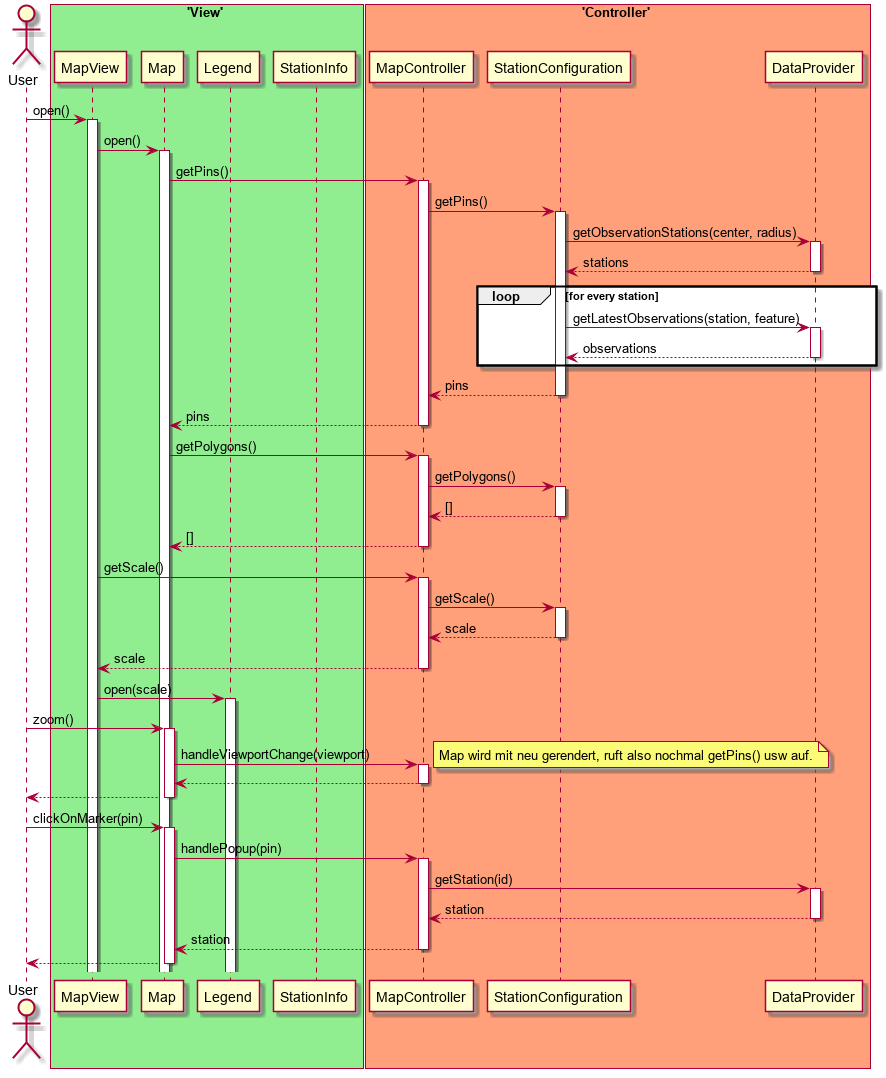
\includegraphics[width=\textwidth,keepaspectratio]{diagrams/MapPageSeq.png}

\newpage
\subsubsection*{Detailansicht}
Das folgende Sequenzdiagramm zeigt das Laden der \gls{Detailansicht}. Einzelne Komponenten werden mit Modellobjekten über ihre props initialisiert. Das ObservationStations Objekt gibt die Diagramme zurück, die angezeigt werden.\\


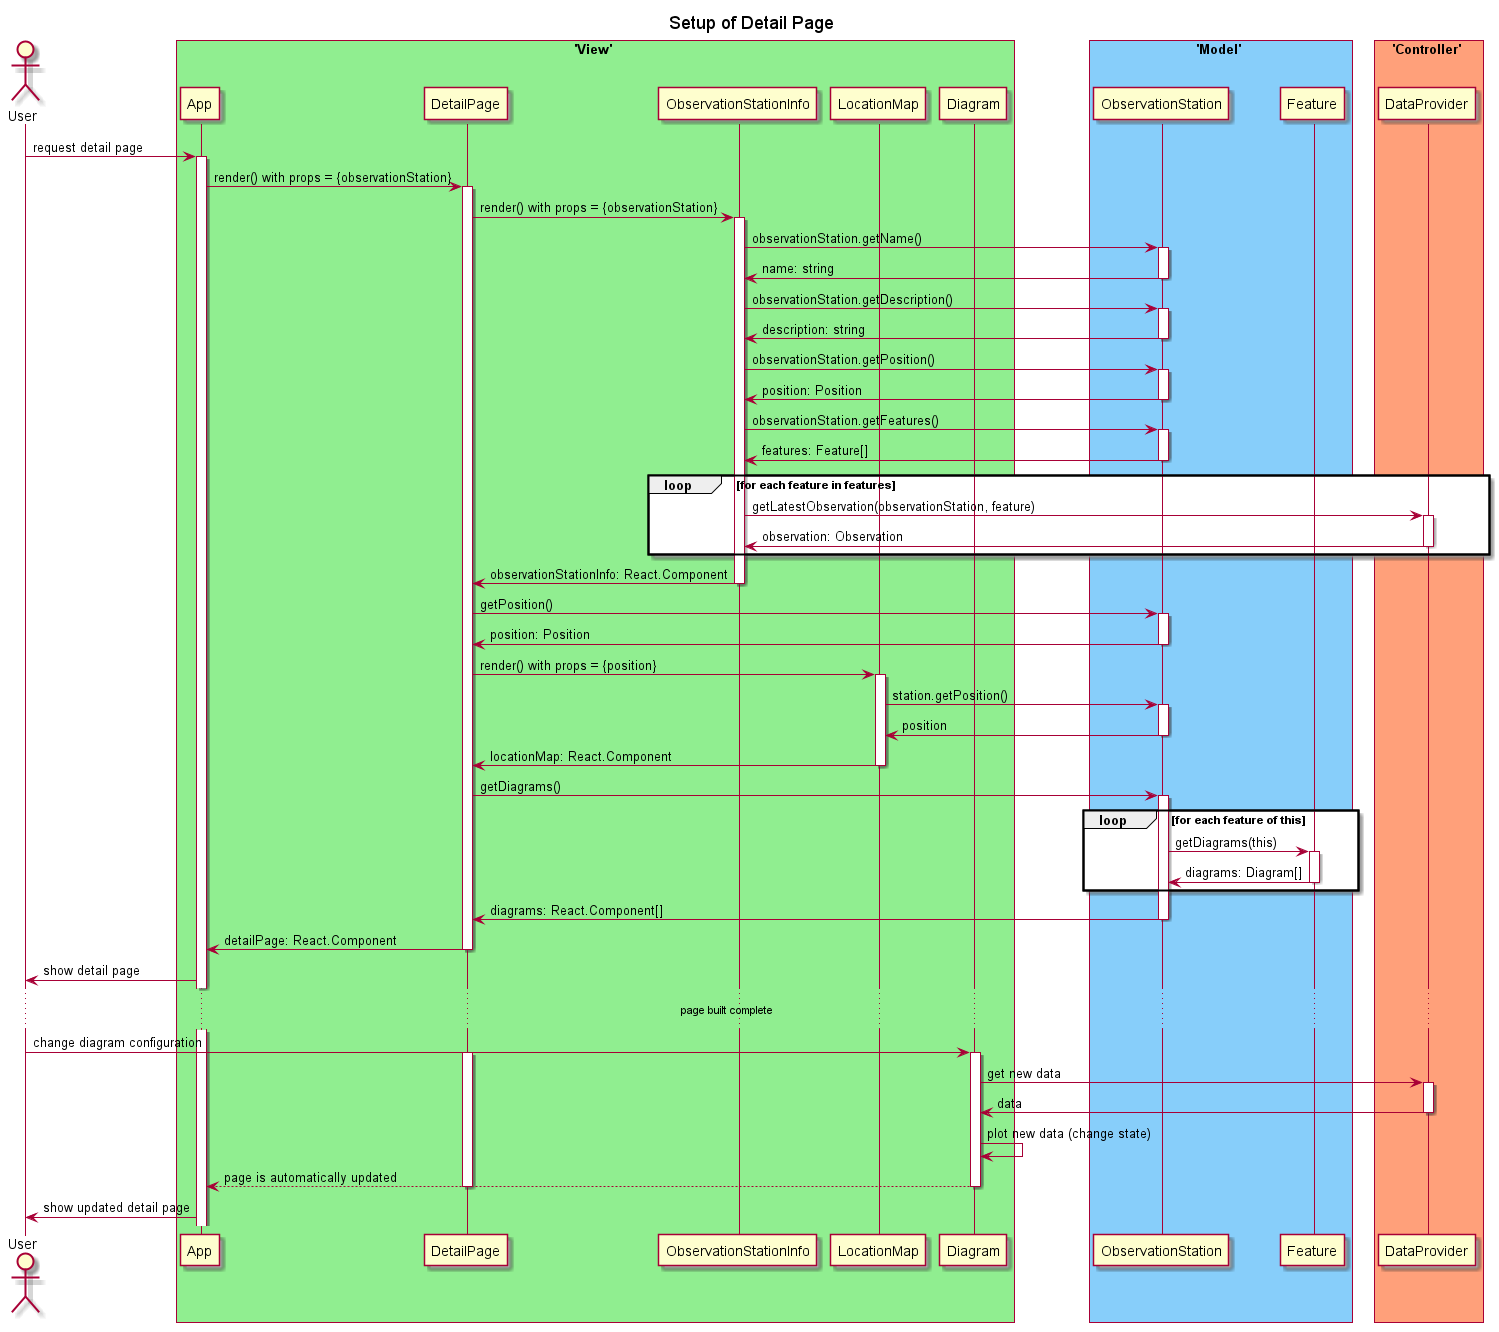
\includegraphics[width=\textwidth,keepaspectratio]{diagrams/DetailPageSeq.png}

\newpage
\subsubsection*{FROST}
Das folgende Sequenzdiagramm zeigt exemplarisch den FROST-package internen Ablauf bei Aufruf der getObservationStations-Methode von DataProvider.\\


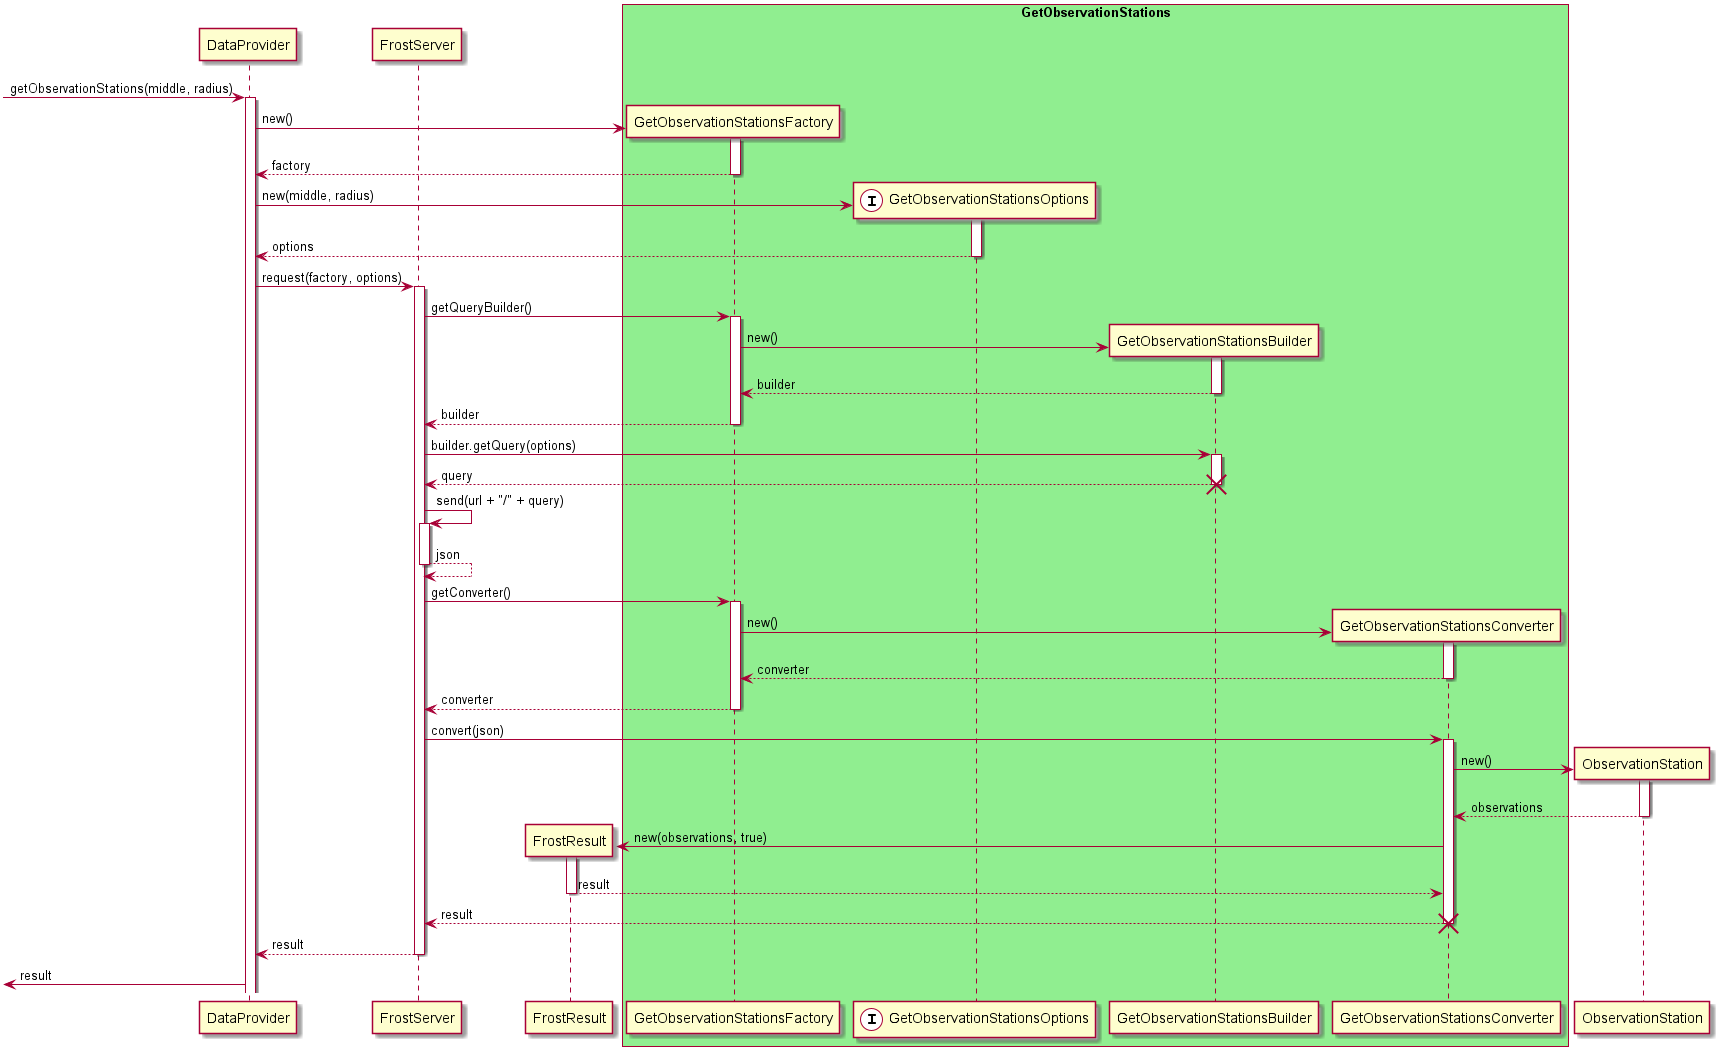
\includegraphics[width=\textwidth,keepaspectratio]{diagrams/FrostFactory.png}